\section{Messaging}
\label{sec:messaging}

% custom message commands
\newcommand{\messagefield}[3]{
	\draw[] (0, #3 + 0.25) node[label=left:\small{#1}]{};
	\draw[draw=black] (0, #3) rectangle (4, #3 + 0.5);
	\draw[] (2, #3 + 0.25) node[label=center:\small{#2}]{};
}

\nemquote{
}{}

\nemchapterfirstletter{B}{lockchain} client applications retrieve blockchain data and present it to their users.
In order for these clients to be most useful, they should always present the most up to date blockchain data and refresh their user interfaces whenever the displayed data changes.
A naive client could periodically poll a REST server or a local database for blockchain data.
This is inefficient because it requires using more network bandwidth and other resources than necessary.
Instead, \codenamespace allows clients to subscribe to data changes via a single message queue.

\subsection{Message Channels And Topics}
\index{messaging!channels}
\label{sec:messaging:channels}

The \codenamespace message queue exposed to clients supports multiple channels.
Each channel has a unique \emph{topic}.
A topic always starts with a topic marker that indicates the kind of messages that will be received.
In some cases, the marker is followed by an unresolved address that is used for additional filtering.
Since a client is usually not interested in every type of blockchain state change, it can subscribe to a subset of available topics.
\autoref{tbl:messaging:topicMarkers} lists all supported topic markers.

\begin{figure}[H]
	\nemcenterwithcaption{
		\begin{tabular}{|l|c|}
			\hline
			\rule{0pt}{20pt}\textbf{Topic marker name} & \textbf{Topic marker}\\[1.2ex]
			\hline
			Block & 0x9FF2D8E480CA6A49\\
			\hline
			Drop blocks & 0x5C20D68AEE25B0B0\\
			\hline
			Transaction & 0x61\\
			\hline
			Unconfirmed transaction add & 0x75\\
			\hline
			Unconfirmed transaction remove & 0x72\\
			\hline
			Partial transaction add & 0x70\\
			\hline
			Partial transaction remove & 0x71\\
			\hline
			Transaction status & 0x73\\
			\hline
			Cosignature & 0x63\\
			\hline
		\end{tabular}
	}{Topic Markers}
	\label{tbl:messaging:topicMarkers}
\end{figure}

\subsection{Connection And Subscriptions}
\index{messaging!messages}
\label{sec:messaging:messages}

Support for messaging is added by the zeromq extension.
If a node wants to support messaging, this extension must be enabled in the broker process.
The extension registers subscribers for block and transaction related events \nemrefparens{sec:system:extensions} and maps those events to message queue messages.
When enabled, the broker listens on port \nemsetting{messaging}{subscriberPort} for new subscribers.
Clients can connect and subscribe to the message queue for one or more topics.

\subsection{Block Messages}

The topics for block messages only consist of a topic marker.
The layouts for all block messages are displayed in \autoref{fig:messaging:blockMessages}.
The following block messages are supported:

\begin{itemize}
	\item{Block: A new block was added to the chain.}
	\item{Drop blocks: Blocks after a given height were dropped.}
\end{itemize}

\begin{figure}[H]
	\nemcenterwithcaption{
		\begin{subfigure}{.5\textwidth}
			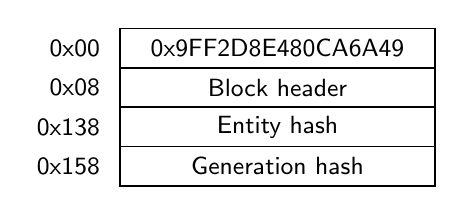
\begin{tikzpicture}[>=latex,font=\sffamily,semithick]
				\messagefield{0x00}{0x9FF2D8E480CA6A49}{0.0}
				\messagefield{0x08}{Block header}{-0.5}
				\messagefield{0x138}{Entity hash}{-1.0}
				\messagefield{0x158}{Generation hash}{-1.5}
			\end{tikzpicture}
			\caption{Block message layout}
		\end{subfigure}%
		\begin{subfigure}{.5\textwidth}
			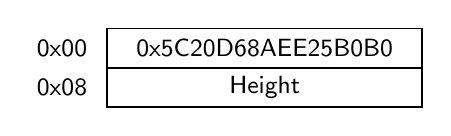
\begin{tikzpicture}[>=latex,font=\sffamily,semithick]
				\messagefield{0x00}{0x5C20D68AEE25B0B0}{0.0}
				\messagefield{0x08}{Height}{-0.5}
			\end{tikzpicture}
			\caption{Drop blocks message layout}
		\end{subfigure}
	}{Block related messages}
	\label{fig:messaging:blockMessages}
\end{figure}

\subsection{Transaction Messages}

The topics for transaction messages consist of both a topic marker and an optional unresolved address filter.
When an unresolved address filter is supplied, only messages that involve the specified unresolved address will be raised.
For example, a message will be raised for a transfer transaction only if the specified unresolved address is the sender or the recipient of the transfer.
When no unresolved address filter is supplied, messages will be raised for all transactions.
The layouts for all transaction messages are displayed in \autoref{fig:messaging:unconfirmedTransactionMessages} , \autoref{fig:messaging:partialTransactionMessages} and \autoref{fig:messaging:transactionStatusMessage}.
The following transaction messages are supported:

\begin{itemize}
	\item{Transaction: A transaction was confirmed, i.e. is part of a block.}
	\item{Unconfirmed transaction add: An unconfirmed transaction was added to the unconfirmed transactions cache.}
	\item{Unconfirmed transaction remove: An unconfirmed transaction was removed from the unconfirmed transactions cache.}
	\item{Partial transaction add: A partial transaction was added to the partial transactions cache.}
	\item{Partial transaction remove: A partial transaction was removed from the partial transactions cache.}
	\item{Transaction status: The status of a transaction changed.}
\end{itemize}

\begin{figure}[H]
	\nemcenterwithcaption{
		\begin{subfigure}{.5\textwidth}
			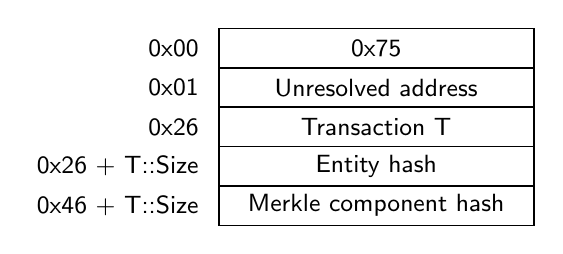
\begin{tikzpicture}[>=latex,font=\sffamily,semithick]
				\messagefield{0x00}{0x75}{0.0}
				\messagefield{0x01}{Unresolved address}{-0.5}
				\messagefield{0x26}{Transaction T}{-1}
				\messagefield{0x26 + T::Size}{Entity hash}{-1.5}
				\messagefield{0x46 + T::Size}{Merkle component hash}{-2}
			\end{tikzpicture}
			\caption{Add message}
		\end{subfigure}%
		\begin{subfigure}{.5\textwidth}
			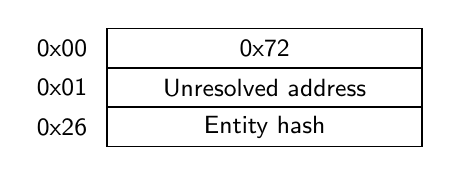
\begin{tikzpicture}[>=latex,font=\sffamily,semithick]
				\messagefield{0x00}{0x72}{0.0}
				\messagefield{0x01}{Unresolved address}{-0.5}
				\messagefield{0x26}{Entity hash}{-1.0}
			\end{tikzpicture}
			\caption{Remove message}
		\end{subfigure}%
	}{Unconfirmed transactions related messages}
	\label{fig:messaging:unconfirmedTransactionMessages}
\end{figure}

\begin{figure}[H]
	\nemcenterwithcaption{
		\begin{subfigure}{.5\textwidth}
			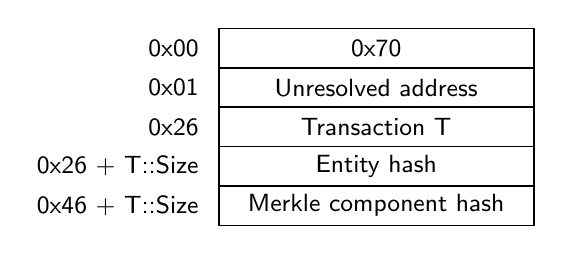
\begin{tikzpicture}[>=latex,font=\sffamily,semithick]
				\messagefield{0x00}{0x70}{0.0}
				\messagefield{0x01}{Unresolved address}{-0.5}
				\messagefield{0x26}{Transaction T}{-1}
				\messagefield{0x26 + T::Size}{Entity hash}{-1.5}
				\messagefield{0x46 + T::Size}{Merkle component hash}{-2}
			\end{tikzpicture}
			\caption{Add message}
		\end{subfigure}%
		\begin{subfigure}{.5\textwidth}
			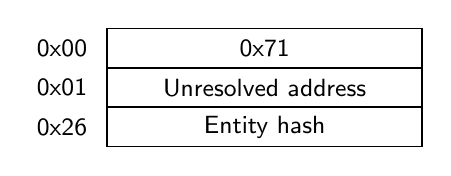
\begin{tikzpicture}[>=latex,font=\sffamily,semithick]
				\messagefield{0x00}{0x71}{0.0}
				\messagefield{0x01}{Unresolved address}{-0.5}
				\messagefield{0x26}{Entity hash}{-1.0}
			\end{tikzpicture}
			\caption{Remove message}
		\end{subfigure}%
	}{Partial transactions related messages}
	\label{fig:messaging:partialTransactionMessages}
\end{figure}

\begin{figure}[H]
	\nemcenterwithcaption{
		\begin{subfigure}{.5\textwidth}
			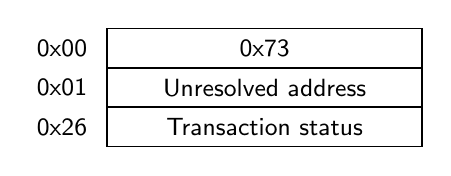
\begin{tikzpicture}[>=latex,font=\sffamily,semithick]
				\messagefield{0x00}{0x73}{0.0}
				\messagefield{0x01}{Unresolved address}{-0.5}
				\messagefield{0x26}{Transaction status}{-1}
			\end{tikzpicture}
			\caption{Add message}
		\end{subfigure}%
	}{Transaction status message}
	\label{fig:messaging:transactionStatusMessage}
\end{figure}

\subsubsection{Cosignature Message}

The topic for a cosignature message consists of both a topic marker and an optional unresolved address filter.
The message is emitted to the subscribed clients when a new cosignature for an aggregate transaction is added to the partial transactions cache.
When an unresolved address filter is supplied, messages will only be raised for aggregate transactions that involve the specified address.
Otherwise, messages will be raised for all changes.
The layout for the cosignature message is displayed in \autoref{fig:messaging:cosignatureMessage}.

\begin{figure}[H]
	\nemcenterwithcaption{
		\begin{subfigure}{.5\textwidth}
			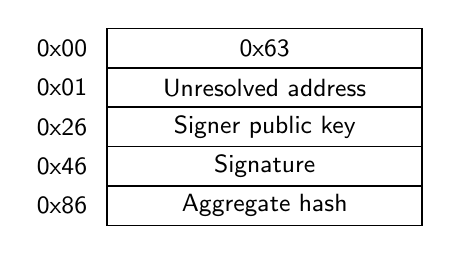
\begin{tikzpicture}[>=latex,font=\sffamily,semithick]
				\messagefield{0x00}{0x63}{0.0}
				\messagefield{0x01}{Unresolved address}{-0.5}
				\messagefield{0x26}{Signer public key}{-1}
				\messagefield{0x46}{Signature}{-1.5}
				\messagefield{0x86}{Aggregate hash}{-2}
			\end{tikzpicture}
		\end{subfigure}%
	}{Cosignature message}
	\label{fig:messaging:cosignatureMessage}
\end{figure}
